% The packages used here are just a sample. You may need others, and may not need some of these. It doesn't hurt to leave them in, unless they start to conflict with other packages you've added. Chapter 2 has example code for equations, figures, tables, citations, abbreviations, etc. If there are sections labeled 'optional' that you don't want, just comment them out. -jg

\documentclass[reqno,12pt,oneside]{report} % right-side equation numbering, 12 point font, print one-sided 
%\documentclass[reqno,12pt,twoside,openright]{report} % right-side equation numbering, 12 point font, print two-sided, Chapters start on odd pages. Rackham only accepts one-sided, so this is for personal printings.

\usepackage{rac}         % Use Rackham thesis style file
\usepackage{aas_macros}  % To allow the reading of ADS journal references in the bibliography
\usepackage[intlimits]{amsmath} % Puts the limits of integrals on top and bottom
\usepackage{amsxtra}     % Use various AMS packages
\usepackage{amsthm}
\usepackage{amssymb}
\usepackage{amsfonts}
\usepackage{graphicx}    % Add some packages for figures. Read epslatex.pdf on ctan.tug.org
\usepackage{rotating}
\usepackage{color}
\usepackage{epsfig}
\usepackage{subfigure}   % To make subfigures. Read subfigure.pdf on ctan.tug.org
\usepackage{verbatim}
\usepackage{natbib}      % Allows you to use BibTeX
\usepackage[printonlyused]{acronym} % For the List of Abbreviations. Read acronym.pdf on ctan.tug.org
\usepackage{setspace}    % Allows you to specify the line spacing
\doublespacing           % \onehalfspacing for 1.5 spacing, \doublespacing for 2.0 spacing.
\newcommand{\sun}{\ensuremath{\odot}} % sun symbol is \sun
%%%%%%%%%%%%%%%%%%%%%%%%%%%%%%%%%%%%%%%%%%%%%%%%%%%%%%%%%%%%%%%%%%%%%%%%%%%%%%%

% Various theorem environments. All of the following have the same numbering
% system as theorem.

\theoremstyle{plain}
\newtheorem{theorem}{Theorem}
\newtheorem{prop}[theorem]{Proposition}
\newtheorem{corollary}[theorem]{Corollary}
\newtheorem{lemma}[theorem]{Lemma}
\newtheorem{question}[theorem]{Question}
\newtheorem{conjecture}[theorem]{Conjecture}
\newtheorem{assumption}[theorem]{Assumption}

\theoremstyle{definition}
\newtheorem{definition}[theorem]{Definition}
\newtheorem{notation}[theorem]{Notation}
\newtheorem{condition}[theorem]{Condition}
\newtheorem{example}[theorem]{Example}
\newtheorem{introduction}[theorem]{Introduction}

\theoremstyle{remark}
\newtheorem{remark}[theorem]{Remark}
%%%%%%%%%%%%%%%%%%%%%%%%%%%%%%%%%%%%%%%%%%%%%%%%%%%%%%%%%%%%%%%%%%%%%%%%%%%%%%%

\numberwithin{theorem}{chapter}     % Numbers theorems "x.y" where x
                                    % is the section number, y is the
                                    % theorem number

%\renewcommand{\thetheorem}{\arabic{chapter}.\arabic{theorem}}

%\makeatletter                      % This sequence of commands will
%\let\c@equation\c@theorem          % incorporate equation numbering
%\makeatother                       % into the theorem numbering scheme

%\renewcommand{\theenumi}{(\roman{enumi})}

%%%%%%%%%%%%%%%%%%%%%%%%%%%%%%%%%%%%%%%%%%%%%%%%%%%%%%%%%%%%%%%%%%%%%%%%%%%%%%

% If printing two-sided, this makes sure that any blank page at the 
% end of a chapter will not have a page number. 
\makeatletter
\def\cleardoublepage{\clearpage\if@twoside \ifodd\c@page\else
\hbox{}
\thispagestyle{empty}
\newpage
\if@twocolumn\hbox{}\newpage\fi\fi\fi}
\makeatother 

%%%%%%%%%%%%%%%%%%%%%%%%%%%%%%%%%%%%%%%%%%%%%%%%%%%%%%%%%%%%%%%%%%%%%%%%%%%%%%

%This command creates a box marked ``To Do'' around text.
%To use type \todo{  insert text here  }.

\newcommand{\todo}[1]{\vspace{5 mm}\par \noindent
\marginpar{\textsc{To Do}}
\framebox{\begin{minipage}[c]{0.95 \textwidth}
\tt\begin{center} #1 \end{center}\end{minipage}}\vspace{5 mm}\par}

%%%%%%%%%%%%%%%%%%%%%%%%%%%%%%%%%%%%%%%%%%%%%%%%%%%%%%%%%%%%%%%%%%%%%%%%%%%%%%%
\begin{document}

\bibliographystyle{agu04}    % Set the bibliography style. agu04, plain, alpha, etc.

% Title page as required by Rackham dissertation guidelines
\titlepage{Heterogeneous Memory Management}{Neha Agarwal}{Doctor of Philosophy}
{Computer Science and Engineering}{2015}
{Associate Professor Thomas F. Wenisch, Chair\\
 Professor Peter M. Chen\\
 Assistant Professor Ronald G. Dreslinski\\
 Assistant Professor cognate}

% Begin the front matter as required by Rackham dissertation guidelines
\initializefrontsections

% Optional Frontispiece
\frontispiece{
\includegraphics[width=6in]{Intro/Happy} Find a cool picture to go here.}

% Optional, but recommended, Copyright page
\copyrightpage{Your Name}

% Page numbering. If you don't include a frontispiece or copyright page, you'll need to change this for two-sided printing.
\makeatletter
\if@twoside \setcounter{page}{4} \else \setcounter{page}{1} \fi
\makeatother
 
% Optional Dedication page
\dedicationpage{For all the people}

% Optional Acknowledgements page
\startacknowledgementspage
Thanks to the people who made this dissertation possible, especially those who put together a nice \LaTeX\, template for me to use.
\label{Acknowledgements}

% Optional Preface page
%\startprefacepage
%\input{Preface}
%\label{Preface}

% Table of contents, list of figures, etc.
\tableofcontents     % Required
\listoffigures       % Required if there is more than one figure
%\listoftables        % Required if there is more than one table
%\listofmaps          % Required if there is more than one map
%\listofappendices    % Required if there is more than one appendix
\listofabbreviations % Optional. Abbreviations should be stored in a file named abbr.tex

% Optional in-dissertation Abstract Page
\startabstractpage
{Heterogeneous Memory Management}{Neha Agarwal}{Chair: Thomas F. Wenisch}
This template conforms to University of Michigan abstract and dissertation format guidelines as of September 2008. It is an update to a template that has been floating around among grad students here for about 20 years. The main components are the thesis.tex file and the rac.sty file, the latter of which should not need any modification. If BibTeX is used (and for a dissertation, it should be), then References.bib is also needed. If a list of acronyms is desired, make all additions in abbr.tex and read acronym.pdf on ctan.org for details on how to call them in the text. Other files in this template that may be helpful, but don't necessarily need to be used include a style file that formats your bibliography in AGU format (agu04.bst) and a style file that allows you to use abbreviations for journal names (aas\_macros.sty) when typing out the bibliography. This will be necessary if you grab BibTeX information from places like the NASA ADS, which sometimes uses journal name abbreviations. It is useful to separate chapters into their own subfolders, with each folder containing the chapter's .tex file as well as all associated figures. For the figures, just call the name of the file, without the suffix (i.e., includegraphics\{Chap5/LabSetup\}) and the graphicx package will figure out what type of file it is. To compile to pdf, some format other than .eps must be used with the figures. To compile to ps, the figures need to be in ps or eps. If using \LaTeX\, in a Windows environment, there are several different editors and programs that can be used. One set that is known to work well is the following, which can each be found with a simple web search and which should be installed in this order: a Perl distribution such as ActivePerl, a \TeX\, distribution such as MikTex, a \LaTeX\, editor such as TeXnicCenter, a postscript interpreter like Ghostscript, and a postscript viewer like GSView. I included a few pages of sample code in chapter 2 to help you get started, including code for writing equations, citations, abbreviations, tables, and calling graphics. Always be sure to compile your thesis.tex file a couple of times to get the references and page numbering updated. Good luck. -jg
\label{Abstract}

\startthechapters 
% The individual files for each of the chapters are put here.
% Save each chapter of your thesis to a seperate tex file
% and then use the \input command to include this file in your
% thesis.  For instance you can save a file to "intro.tex" and 
% then type %{\color{red}
%\begin{itemize}
%\item New memory technologies
%\item Why is virtual address shared space is a challenge with the advent of
%these new technologies
%
%\item How is CPU--GPU space changing in terms
%of high bandwidth but lower latency interconnects
%\item Present opportunities and challenges
%\item Combine intro of first 3 GPU papers
%
%\item Google Proposal
%\item How cheaper but slower mem technologies can lead to boosting perf/dollar
%in data-centers
%\item Present opportunities and challenges
%\end{itemize}
%}
%
The emergence of {\it heterogeneous memory systems} has resulted in a need for
new memory management policies that are able to fully exploit these systems.
While traditional memory management techniques largely assume a ``homogeneous''
main memory, future systems are likely to have two or more different types of
main memories attached to them -- thus the term ``heterogeneous'' memory
systems. An example of such system is the recently announced NVIDIA's Pascal
GPU~\cite{pascal}, which is slated to have high bandwidth connection to the host
CPU by NVLink~\cite{NVLINK} and thus can access host memory seamlessly.  Another
example is Intel's 3-D XPoint technology~\cite{xpoint}, which provides a slow
but cheaper and large capacity non-volatile memory (NVRAM) along with a regular
DRAM based memory attached to the same CPU node.  There are several aspects of
such systems that have not been studied before:

\begin{enumerate}
\item
\textbf{Different bandwidths:}
Different memory technologies will typically have differences in their
bandwidths, e.g., a GPU connected to on-board GDDR and host-side DDR memories
can have a bandwidth differential of $\approx$ 2 -- 8 $\times$ between the two
memory technologies. Since GPUs are sensitive to main memory bandwidth, the
metric to optimize for in such systems is the total available bandwidth to the
GPU from the two memory sources. While prior work on Non-Uniform Memory Access
(NUMA) has closely looked at data placement strategies to optimize the total
memory {\it access latency} in the presence of different memory zones with
different access latencies, we show that such policies are not suited to
optimizing the total memory {\it bandwidth}. Instead, we propose {\it
Bandwidth-Aware Placement} (BW-AWARE), which directly maximizes the overall
bandwidth, and show that it can significantly increase application throughput
for several GPU applications.

\item
\textbf{Different coherency domains:} 
In a heterogeneous CPU-GPU memory system, implementing hardware cache coherence
between the CPU and the GPU can lead to a significant challenges because of
design and verification involved particularly if the two domains are designed by
separate vendors. We introduce {\it Selective Caching}, a coherence policy that
disallows GPU caching of any memory that would require coherence updates to
propagate across the two domains. This approach decouples the cache-coherence
protocols in CPUs and GPUs, thus improving cross-vendor design cycle time.

\item
\textbf{Different costs per bit:}
Different memory technologies can have different costs.  For example, recently
announced non-volatile memory technology~\cite{xpoint} is projected to be
significantly cheaper than regular DRAM, while also being significantly higher
latency. Their lower cost per bit makes them a good candidate for use in
data-centers, where main memory cost can be up to $\approx$ 30\% of the total
cost of ownership (TCO). However, their low speed means that only {\it cold},
i.e., infrequently accessed data can be placed in such memories. However, placing more
cold data in the slower memories conflicts with efficient virtual memory usage
by transparent huge page (THP), which can provide 10-15\% performance gains in
large memory footprint data-center applications. We study how to reap the
benefits of huge pages while also placing as much data in slow memory as
possible, to improve performance per dollar in data-centers.
\end{enumerate}

Below, we describe each of these three problems in detail and give a brief
sketch of our proposed solution to these problems.

\section{Bandwidth-asymmetric Systems}
To date, GPU-attached Bandwidth-Optimized (BO) memory has been allocated and
managed primarily as through explicit, programmer-directed function calls.
To make best use of the bandwidth available to GPU programs, programmers
manually copy the data over the relatively slow PCIe bus to the GPU memory, and
--- only then --- launch their GPU kernels.  This up-front data allocation and
transfer has been necessary since transferring data over the PCIe bus is a high
overhead operation, and a bulk transfer of data amortizes this overhead. This
data manipulation overhead also results in significant porting challenges when
retargeting existing applications to GPUs, particularly for high-level languages
that make use of libraries and dynamic memory allocation during application
execution.

\begin{figure}[t]
    \centering
    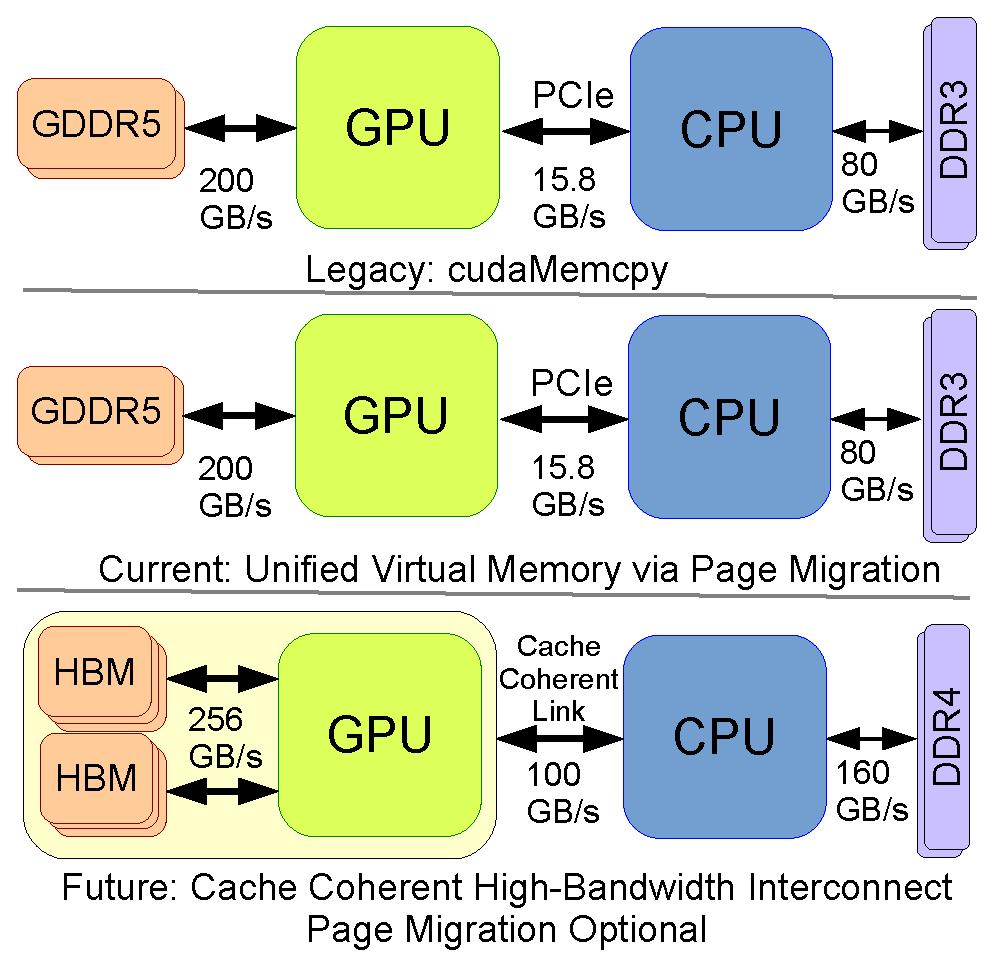
\includegraphics[width=0.7\columnwidth]{hpca2015/figures/architecture.eps}
    \caption{System architectures for legacy, current, and future mixed GPU-CPU systems.}
    \label{fig:arch-hpca2015}
\end{figure}

Recognizing the obstacle this programming model poses to the wider adoption of
GPUs in more parallel applications, programming systems like NVIDIA's CUDA,
OpenCL, and OpenACC are evolving to shared virtual address space between CPU and
GPU~\cite{UVM}. Concurrently, CPU-GPU architectures are evolving to have unified
globally addressable memory systems in which both the GPU and CPU can access any
portion of memory at any time, regardless of its physical location.  Today this
unified view of memory is layered on top of legacy hardware designs by
implementing software-based runtimes that dynamically copy data on demand
between the GPU and CPU~\cite{cuda}. As depicted in
Figure~\ref{fig:arch-hpca2015}, over the next several years it is expected that
GPU and CPU systems will move away from the PCIe interface to a fully cache
coherent (CC) interface ~\cite{AMDHSA}. These systems will provide high
bandwidth ($5-10x$ higher) and low latency ($10x$ lower) between the non-uniform memory
access (NUMA) pools attached to discrete processors by layering coherence
protocols on top of physical link technologies such as NVLink~\cite{NVLINK},
Hypertransport~\cite{AMDHT}, or QPI~\cite{INTELQPI}.   CC-NUMA access to
CPU-attached memory from the GPU makes the software page migration used today an
optional feature thanks to the improved bandwidth, latency, and access
granularity that cache coherence can provides.

As heterogeneous CPU-GPU systems move to a transparent unified memory system,
the OS and runtime systems need information about other aspects of memory zones
such as their bandwidths instead of only the access latency information that is
exposed today via Advanced Configuration and Power Interface (ACPI). In CC-NUMA
systems today, latency information alone is adequate as CPUs are generally more
performance sensitive to memory system latency rather than other memory
characteristics. In contrast, massively parallel GPUs and their highly-threaded
programming models have been designed to gracefully handle long memory
latencies, instead demanding high bandwidth. Unfortunately, differences in
bandwidth capabilities, read versus write performance, and access energy are not
exposed to software; making it difficult for the operating system, runtime, or
programmer to make good decisions about memory placement in these GPU-equipped
systems. In this thesis we investigate the effect on GPU performance of exposing
memory system bandwidth information to the operating system/runtime and user
applications to improve the quality of dynamic page placement and migration
decisions.

\section{Different Coherence Domains}
%Technology trends indicate an increasing number of systems designed with CPUs,
%accelerators, and GPUs coupled via high-speed links. Such systems are likely to
%introduce unified shared CPU-GPU memory with shared page tables. In fact, some
%systems already feature such implementations~\cite{AMDKaveri}.
Introducing globally visible shared memory improves programmer productivity by
eliminating explicit copies and memory management overheads. Whereas this
abstraction can be supported using only software page-level protection
mechanisms~\cite{UVM, HSA}, hardware cache coherence can improve performance by
allowing concurrent, fine-grained access to memory by both CPU and GPU.
%If the CPU and GPU have separate physical memories, page migration may also be
%used to optimize page placement for latency or bandwidth by using both near and
%far memory~\cite{Dashti2013,Agarwal2015b,Meswani2015,Chou2015}.

%Some CPU--GPU systems will be tightly integrated into a system on chip (SoC)
%making on-chip hardware coherence a natural fit, possibly even by sharing a
%portion of the on-chip cache hierarchy~\cite{HSA,AMDAPU,Hechtman2014}.  However,
%the largest GPU implementations consume nearly 8B transistors and have their own
%specialized memory systems~\cite{NVIDIA8BILLION}.  Power and thermal constraints
%preclude single-die integration of such designs.  Thus, many CPU--GPU systems
%are likely to have discrete CPUs and GPUs connected via dedicated off-chip
%interconnects like NVLINK (NVIDIA), CAPI (IBM), HT (AMD), and QPI (INTEL) or
%implemented as multi-chip modules~\cite{NVLINK,CAPI,AMDHT,INTELQPI,Chen92}.
%The availability of these high speed off-chip interconnects has led both
%academic groups and vendors like NVIDIA to investigate how future GPUs may
%integrate into existing OS controlled unified shared memory regimes used by
%CPUs~\cite{Pichai2014,Power2014,Agarwal2015,Agarwal2015b}.

Despite the programmability benefits of CPU-GPU cache coherence, designing such
a system can involve several hurdles. Prior studies~\cite{Hong2012} have shown
that coherence implementations are a major source of hardware design bugs.
Extending a CPU coherence implementation to a GPU over a long-latency
interconnect ($approx$ 100ns)  will only increase the design cost of such a system.
Also, if the CPUs and GPUs are to be manufactured by different vendors, a high
level of coordination has to be done between those two vendors -- including
coordination on the specification of coherence implementation and verification
efforts. Such hurdles make CPU-GPU cache coherence an unattractive option to
deploy in a product.

Current CPUs have up to 18 cores per socket~\cite{INTELXEONE5V3} but GPUs are
expected to have hundreds of streaming multiprocessors (SMs) each with its own
cache(s) within the next few years. Hence, extending traditional hardware
cache-coherency into a multi-chip CPU-GPU memory system requires coherence
messages to be exchanged not just within the GPU but over the CPU-GPU
interconnect. Keeping these hundreds of caches coherent with a traditional HW
coherence protocol, as shown in Figure~\ref{fig:motivation}, potentially
requires large state and interconnect bandwidth~\cite{Kelm2010,johnson2011}.
Some recent proposals call for data-race-free GPU programming models, which
allow relaxed or scoped memory consistency to reduce the frequency or hide the
latency of enforcing coherence~\cite{Hechtman2014}.  However, irrespective of
memory ordering requirements, such approaches still rely on hardware
cache-coherence mechanisms to  avoid the need for software to explicitly track
and flush modified cache lines to an appropriate scope at each synchronization
point. Techniques like region coherence~\cite{Power2013} seek to scale coherence
protocols for heterogeneous systems, but require pervasive changes throughout
the CPU and GPU memory systems.
%Such approaches also incur highly coordinated design and verification effort by
%both CPU and GPU vendors~\cite{Hong2012} that is challenging when multiple
%vendors wish to integrate existing CPU and GPU designs in a timely manner.

Due to the significant challenges associated with building such cache-coherent
systems, in this thesis, we architect a GPU \textit{selective caching}
mechanism.  This mechanism provides the conceptual simplicity of CPU-GPU
hardware cache coherence and maintains a high level of GPU performance (93\% of
hardware cache-coherent system), but does not actually implement hardware cache
coherence between the CPU and GPU.
%In our proposed selective caching GPU, the GPU does not cache data that resides
%in CPU physical memory, nor does it cache data that resides in the GPU memory
%that is actively in-use by the CPU on-chip caches.
%This approach is orthogonal to the memory consistency model and leverages the
%latency tolerant nature of GPU architectures combined with upcoming low-latency
%and high-bandwidth interconnects to enable the benefits of shared memory.

\section{Proposal: Cheaper Memory Technologies}
Upcoming memory technologies, such as Intel's recently-announced XPoint-3D
memory~\cite{xpoint}, are projected to be $10x$ denser and $2x$ cheaper per
bit than DRAM while providing the byte-addressable load-store interface of
conventional main memory.  Improved capacity and cost per bit comes at the price
of higher access latency, projected to fall somewhere in the range of 500ns to
several microseconds.  The impending commercial availability of such devices has
renewed interest in two-tiered physical memory, wherein part of a system's
physical address space is implemented with the slower, cheaper memory
technology.  Slow memory can result in a net TCO win if the cost savings of
replaced DRAM outweigh cost increase due to reduced program performance or by
enabling a higher peak memory capacity per server than is economically viable
with DRAM alone.  

%Our preliminary results indicate that over half of the memory footprint of
%representative cloud applications (e.g., Cassandra) are identified as cold by
%Linux’s kstaled mechanism, indicating that the corresponding pages have an
%inter-access interval exceeding 120s.  Analytic modeling suggests these pages
%could be shifted to a memory with a 3us access time with negligible (<3\%)
%performance degradation.

%%It's an interesting problem
%Prior academic work has considered two approaches to two-tiered memory: via a
%paging mechanism~\cite{1,2}, wherein accesses to slow memory invoke a page fault that
%must transfer data to fast memory before an access may proceed, and via a
%migration mechanism (as in cache coherent NUMA multiprocessors)~\cite{XXX}, wherein no
%software fault is required.  In the latter scenario, a migration mechanism seeks
%to shuffle pages between tiers to maximize fast-memory accesses.  

%It's an unsolved problem
Prior academic work on two-tiered memory has assumed migration/paging at 4KB
page granularity.  Huge pages, implemented via Linux's Transparent Huge Page
(THP) mechanism, are now ubiquitous and critical for data-center applications,
boosting application performance by 10-15\%.
%Recent work~\cite{JeffPaper} has demonstrated that 2MB huge pages are particularly
%performance-critical under virtualization.  
%For example, our study demonstrates a 20\% throughput improvement for Hadoop and
%a 40\% speedup on random memory probes when using huge pages under
%virtualization.  
However, huge pages thwart prior two-tiered memory proposals for two reasons:
(1) it is too expensive to frequently migrate pages at 2MB granularity, and (2)
hot regions occur within otherwise cold 2MB huge pages can hurt performance if
placed in the slower memory. 

%Here is my idea
We propose to develop a transparent huge-page-aware two-tiered memory solution
that integrates support for dynamic page migration and transparent huge pages,
achieving both the capacity/cost advantages of two-tiered memory and performance
advantages of huge pages.  Our focus is on cloud computing scenarios where a
high-memory-footprint application, such as Cassandra, Aerospike, or MySQL, runs
under virtualization and may co-run with other, competing applications.  Hot
regions within otherwise cold huge pages present a central challenge to our
objective; existing x86-Linux provides no mechanism to carve out a 4KB hot
region within a 2MB cold page.

%So, we propose translation facades, a 4KB
%translation that remaps a portion of a 2MB mapping with an alternate physical
%address or permissions.  Current x86-Linux requires non-overlapping mappings due
%to hard-coded page table structure and because TLB entries are replaced
%independently, hence, an uncached 4KB facade to a cached 2MB translation could
%lead to a mis-translation. We will pursue implementations of translation
%facades along two paths. (1) Hardware support: we will extend x86 page table and
%TLB design to support facades. (2) Virtualization: Our existing study of huge
%pages under virtualization demonstrate that a majority of the benefit can be
%obtained if host pages are 2MB even if guest pages are 4KB.  We will investigate
%if the two-level translation from guest to host to machine addresses can be
%exploited to emulate hardware support for translation facades.

%Bulleted list of contributions
We propose to develop a Linux prototype that will to estimate the properties of
a system with the following properties:

\begin{enumerate}
\item
We will measure hot and cold memory fractions at 4KB granularity and within 2MB
huge pages to measure two-tiered memory opportunity. We will use kstaled (an
optional extension to the Linux kernel that tracks pages that have not been
accessed over a fixed time interval) and BadgerTrap~\cite{badgertrap} (a tool to
intercept TLB misses in software) to facilitate this characterization. 

\item
We will develop methods to track hot and cold memory regions at run-time.  A
key challenge lies in efficiently tracking hot regions within an otherwise-cold
huge page, as kstaled provides visibility only at page granularity.  We propose
to investigate sampling methods, e.g., by probabilistically demoting huge pages
or leveraging performance counter infrastructure. 

\item
We will develop an online migration mechanism that can shift data between
fast and slow memory tiers while the application is concurrently executing.  We
draw experience from existing NUMA migration and THP memory defragmentation. We
will implement the migration mechanism in the Linux kernel.

\item
We will develop translation facades, a mechanism that remaps a
portion of a 2MB mapping with an alternate physical address or permissions
(using BadgerTrap to emulate performance) and investigate novel page table and
TLB organizations to support facades.
\end{enumerate}

\section{Contributions}
In this thesis we make following contributions:

\begin{itemize}
\item
We show that existing CPU-oriented page placement policies are not only 
sub-optimal for placement in GPU-based systems, but simply do not have the 
appropriate information available to make informed decisions when optimizing for 
bandwidth-asymmetric memory systems. Exposing additional bandwidth information 
to the OS, as is done for latency today, will be required for optimized decision 
making.

\item
We show that placing all pages in the bandwidth optimized memory is not the best
performing page placement policy for GPU workloads.  We propose a new
bandwidth-aware (BW-AWARE) page placement policy that can outperform Linux's
current bandwidth-optimized INTERLEAVE placement by 35\% and the default latency
optimized LOCAL allocation policy by as much as 18\%, when the application
footprint fits within bandwidth-optimized memory capacity.  

%\item
%For \emph{memory capacity constrained} systems (i.e. bandwidth-optimized memory
%capacity is insufficient for the workload footprint), we demonstrate that using
%simple application annotations to inform the OS/runtime of hot versus cold data
%structures can outperform the current Linux INTERLEAVE and LOCAL page placement
%policies.  Our annotation based policy combined with bandwidth information can
%outperform these page placement policies by 19\% and 12\% respectively, and get
%within 90\% of oracle page placement performance.

\item
We show that counter-based metrics to determine when to migrate pages from the
CPU to GPU are insufficient for finding an optimal migration policy to exploit
GPU memory bandwidth.  In streaming workloads, where each page may be accessed
only a few times, waiting for $N$ accesses to occur before migrating a page will
actually limit the number of accesses that occur after migration, reducing the
efficacy of the page migration operation.

\item
TLB shootdown and refill overhead can significantly degrade the performance of
any page migration policy for GPUs\@. We show that combining reactive migration
with virtual address locality information to aggressively prefetch pages can
mitigate much of this overhead, resulting in increased GPU throughput (35\%).

%\item
%The legacy intuition to migrate all data to the GPU local memory in an attempt
%to maximize bandwidth fails to leverage the bandwidth available via the new
%CC-NUMA interface.  A page migration policy which is aware of this differential
%and balances migration with CC-NUMA link utilization will outperform either GPU
%or GPU memory being used in isolation.

\item 
We present a software based memory migration system that, on average,
outperforms CC-NUMA based accesses by 1.95$\times$, performs 6\% better than the
legacy CPU to GPU {\tt memcpy} approach by intelligently using both CPU and GPU
memory bandwidth, and comes within 28\% of oracular page placement, all while
maintaining the relaxed memory semantics of modern GPUs.

%\vspace{-.025in}
\item
We propose GPU selective caching, which can provide a CPU--GPU system that
provides a unified shared memory without requiring hardware cache-coherence
protocols within the GPU or between CPU and GPU caches.

\item
We identify that much of the improvement from GPU caches is due to coalescing 
memory accesses that are spatially contiguous within a cache line.  Leveraging
aggressive request coalescing, GPUs can achieve much of the performance benefit
of caching (80\%), without caches.

%\item
%We propose a small on-die CPU cache specifically to handle uncached requests
%that will be issued at sub-cache line granularity from the GPU. This cache helps both 
%shield the CPU memory system from the bandwidth hungry GPU and supports
%improved CPU--GPU interconnect efficiency by implementing variable-sized transfer granularity.

\item
We demonstrate that a large fraction (60\%) of GPU-accessed data is read-only.
Allowing the GPU to cache this data and relying on page protection mechanisms
rather than hardware coherence to ensure correctness closes the performance gap
between a selective caching and hardware cache-coherent GPU for many
applications.
\end{itemize}
. 

 \chapter{Introduction}
 \label{chap:Intro}
 The weather in space can have substantial effects on everything within the Sun's influence, including Earth. Most of the effects of space weather are mitigated by Earth's atmosphere and magnetic field, which form a barrier that much of the plasma in space cannot penetrate. Spacecraft and astronauts, however, risk exposure to potentially harmful radiation. Space weather can directly affect Earth's atmosphere, such as near Earth's poles where the magnetic field is shaped in such a way that the solar wind can interact with the upper atmosphere and create the aurora. Space weather can be dangerous, as storms from the Sun damage spacecraft and cause power outages on Earth. To protect astronauts and spacecraft from harm, an understanding of the fundamental physics behind space weather is vital. There are many unknown pieces to the puzzle, but through research and experimentation the picture is slowly being pieced together. As mankind looks toward further exploration of the Moon and the planets, the ability to forecast and protect humans from the effects of space weather become even more important.

This research examines new techniques and tools that can be used to study crucial pieces of the space weather puzzle. The emphasis is on ions found in the space environment: the solar wind (keV), pickup ions (10--100 keV), and energetic particles (100 keV--GeV). Each of these particle populations is created by a specific set of processes, described briefly in Chapter~\ref{chap:Particles}, and all have trajectories through space that are closely related to the magnetic field of the Sun and the heliosphere. Within the Alfv\'{e}n radius (10--20 R$_\sun$), where the kinetic energy of the solar wind is weaker than the energy density of the Sun's magnetic field, the solar wind is guided by the field's shape and corotates with the Sun. Beyond this radial distance, the electrically charged and highly conductive solar wind controls and shapes the magnetic field, drawing it radially outward into the heliosphere. Energetic particles travel along the lines of magnetic flux that extend from the solar surface to the outermost reaches of the solar system. To a large degree, if the shape and path of the Sun's magnetic field can be accurately mapped, the trajectories of these particles could be inferred. However, such mapping techniques have been elusive, or inaccessible to the broad community.


 \chapter{Particle Transport and Acceleration}
 \label{chap:Particles}
 \section{Introduction}
\label{Transport Intro}
For reference, some common equations and brief overviews of the three categories of particles will be given in this chapter. The Maxwell equations \eqref{Gauss}--\!\,\eqref{Ampere}, the continuity equation for charge density and current density \eqref{continuity}, the Lorentz force equation \eqref{Lorentz}, Newton's second law of motion \eqref{Newton2}, and the \ac{MHD} approximation of Ohm's Law \eqref{Ohm} are each useful for basic plasma physics. Thorough derivations for these and related equations can be found in several textbooks, including \citet{gombosi98} and \citet{jackson99}.

\begin{subequations}
 \begin{align}
  \nabla\cdot\mathbf{E}&=\frac{\rho_e}{\epsilon_0}&\quad\text{Gauss's Law}
  \label{Gauss}\\
  \nabla\times\mathbf{E}&=-\frac{\partial\mathbf{B}}{\partial t}&\quad\text{Faraday's law of induction}
  \label{Faraday}\\
  \nabla\cdot\mathbf{B}&=0&\quad\text{Gauss's law for magnetism}
  \label{Gauss m}\\
  \nabla\times\mathbf{B}&=\mu_0\mathbf{J}+\mu_0\epsilon_0\frac{\partial\mathbf{E}}{\partial t}&\quad\text{Amp\`{e}re's law}
  \label{Ampere}
 \end{align}
\end{subequations}
\begin{align}
 \nabla\cdot\mathbf{J}&=-\frac{\partial\rho_e}{\partial t}&\quad\text{continuity equation}
 \label{continuity}\\
 \mathbf{F}&=q\left(\mathbf{E}+\mathbf{v}\times\mathbf{B}\right)\quad\text{(N)}&\quad\text{Lorentz force}
 \label{Lorentz}\\
 \mathbf{F}&=m\mathbf{a}\quad\text{(N)}&\quad\text{Newton's 2nd law of motion}
 \label{Newton2}\\
 \mathbf{J}&=\sigma\left(\mathbf{E+v\times B}\right)\quad\text{(A m$^{-2}$)}&\quad\text{Ohm's law}
 \label{Ohm}
\end{align}

In these equations, $\epsilon_0$ is the electric constant (also called the permittivity of free space), $\mu_0$ is the magnetic constant (also called the permeability of free space), $\sigma$ is the electrical conductivity, treated here as a constant, $q$ is the charge, $\rho_e$ is the charge density, $m$ is the mass, $\mathbf{J}$ is the electric current density, and $\mathbf{E}$ and $\mathbf{B}$ are the electric and magnetic fields. $\mathbf{F}$, $\mathbf{v}$, and $\mathbf{a}$ represent force, velocity, and acceleration. 

In \ac{MHD}, the fields are induced by plasma motion, so the fields vary on the same time and length scales as the plasma variables. If high frequency variations in the electric field are not included, and only the non-relativistic regime is considered, the displacement current in Amp\`{e}re's law can be neglected, leading to Equation~\ref{AmpereMHD}.
\begin{align}
 \nabla\times\mathbf{B}&=\mu_0\mathbf{J}&&\quad\text{MHD Amp\`{e}re's law}
 \label{AmpereMHD}
\end{align}
\indent By substituting Equation~\ref{Faraday} and the curl of Equation~\ref{AmpereMHD} into the curl of Equation~\ref{Ohm}, $\mathbf{E}$ and $\mathbf{J}$ can be eliminated to derive the magnetic induction equation \eqref{MHDinduction}. The first term on the right describes the resistive diffusion of the magnetic field in the plasma while the second term describes the convection of the magnetic field by the plasma.
\begin{align}
 \frac{\partial\mathbf{B}}{\partial t}=\frac{1}{\sigma\mu_0}\nabla^2\mathbf{B}+\nabla\times\left(\mathbf{v}\times\mathbf{B}\right)&&\quad\text{magnetic induction equation}
 \label{MHDinduction}
\end{align}

Since Equation~\ref{Gauss m} states that the divergence of the magnetic field vector $\mathbf{B}$ is zero, $\mathbf{B}$ can be written in terms of a vector potential $\mathbf{A}$:
\begin{align}
 \mathbf{B}=\nabla\times\mathbf{A}\quad\text{(T)}.
 \label{B field}
\end{align}

By substituting Equation~\ref{B field} into Equation~\ref{Faraday}, Faraday's law of induction can be written as a quantity with a vanishing curl. Such a quantity can be rewritten as the gradient of a scalar function, the scalar potential $\Phi$, leading to an equation for $\mathbf{E}$ in terms of the potentials $\mathbf{A}$ and $\Phi$:
\begin{align}
 \mathbf{E}=-\nabla\Phi-\frac{\partial\mathbf{A}}{\partial t}\quad\text{(V m$^{-1}$)}.
 \label{E field}
\end{align}

For electrostatics, all derivatives with respect to time are zero. In this case, the divergence of Equation~\ref{E field} combined with Equation~\ref{Gauss} will give the Poisson equation, or in the absence of charges, the Laplace equation:
\begin{align}
 \nabla^2\Phi &= -\frac{\rho_e}{\epsilon_0},&\quad\text{Poisson's equation}
 \label{Poisson}\\
 \nabla^2\Phi &= 0.&\quad\text{Laplace's equation}
 \label{Laplace}
\end{align}

Due to the historical precedent of the symbols used in these and other common equations, a symbol may have different meanings depending on the equation in which it is used (i.e., `E' can represent `electric field' or `energy'). Even though the meaning of the symbol can usually be discerned from the context of the equation, an attempt has been made to use distinct symbols throughout this dissertation, or use subscripts to clarify a symbol's meaning when necessary. In the specific case of `E', the bold font $\mathbf{E}$ is used to represent the electric field vector and $\left|\mathbf{E}\right|$  to represent the magnitude of the electric field. The plain font E is always used here to represent energy.

Particle transport and acceleration are important topics of research in heliophysics. An understanding of the composition and nature of the gas and plasma found in space is vital to the forecasting of space weather. This research focuses on ways to investigate three categories of particles: the solar wind (\S~\ref{Solar Wind}), pickup ions, and energetic particles, as shown in Figure~\ref{fig:H_Distribution}. The following is intended to provide sufficient background for the scope of this dissertation research.
\begin{figure}
  \centering
  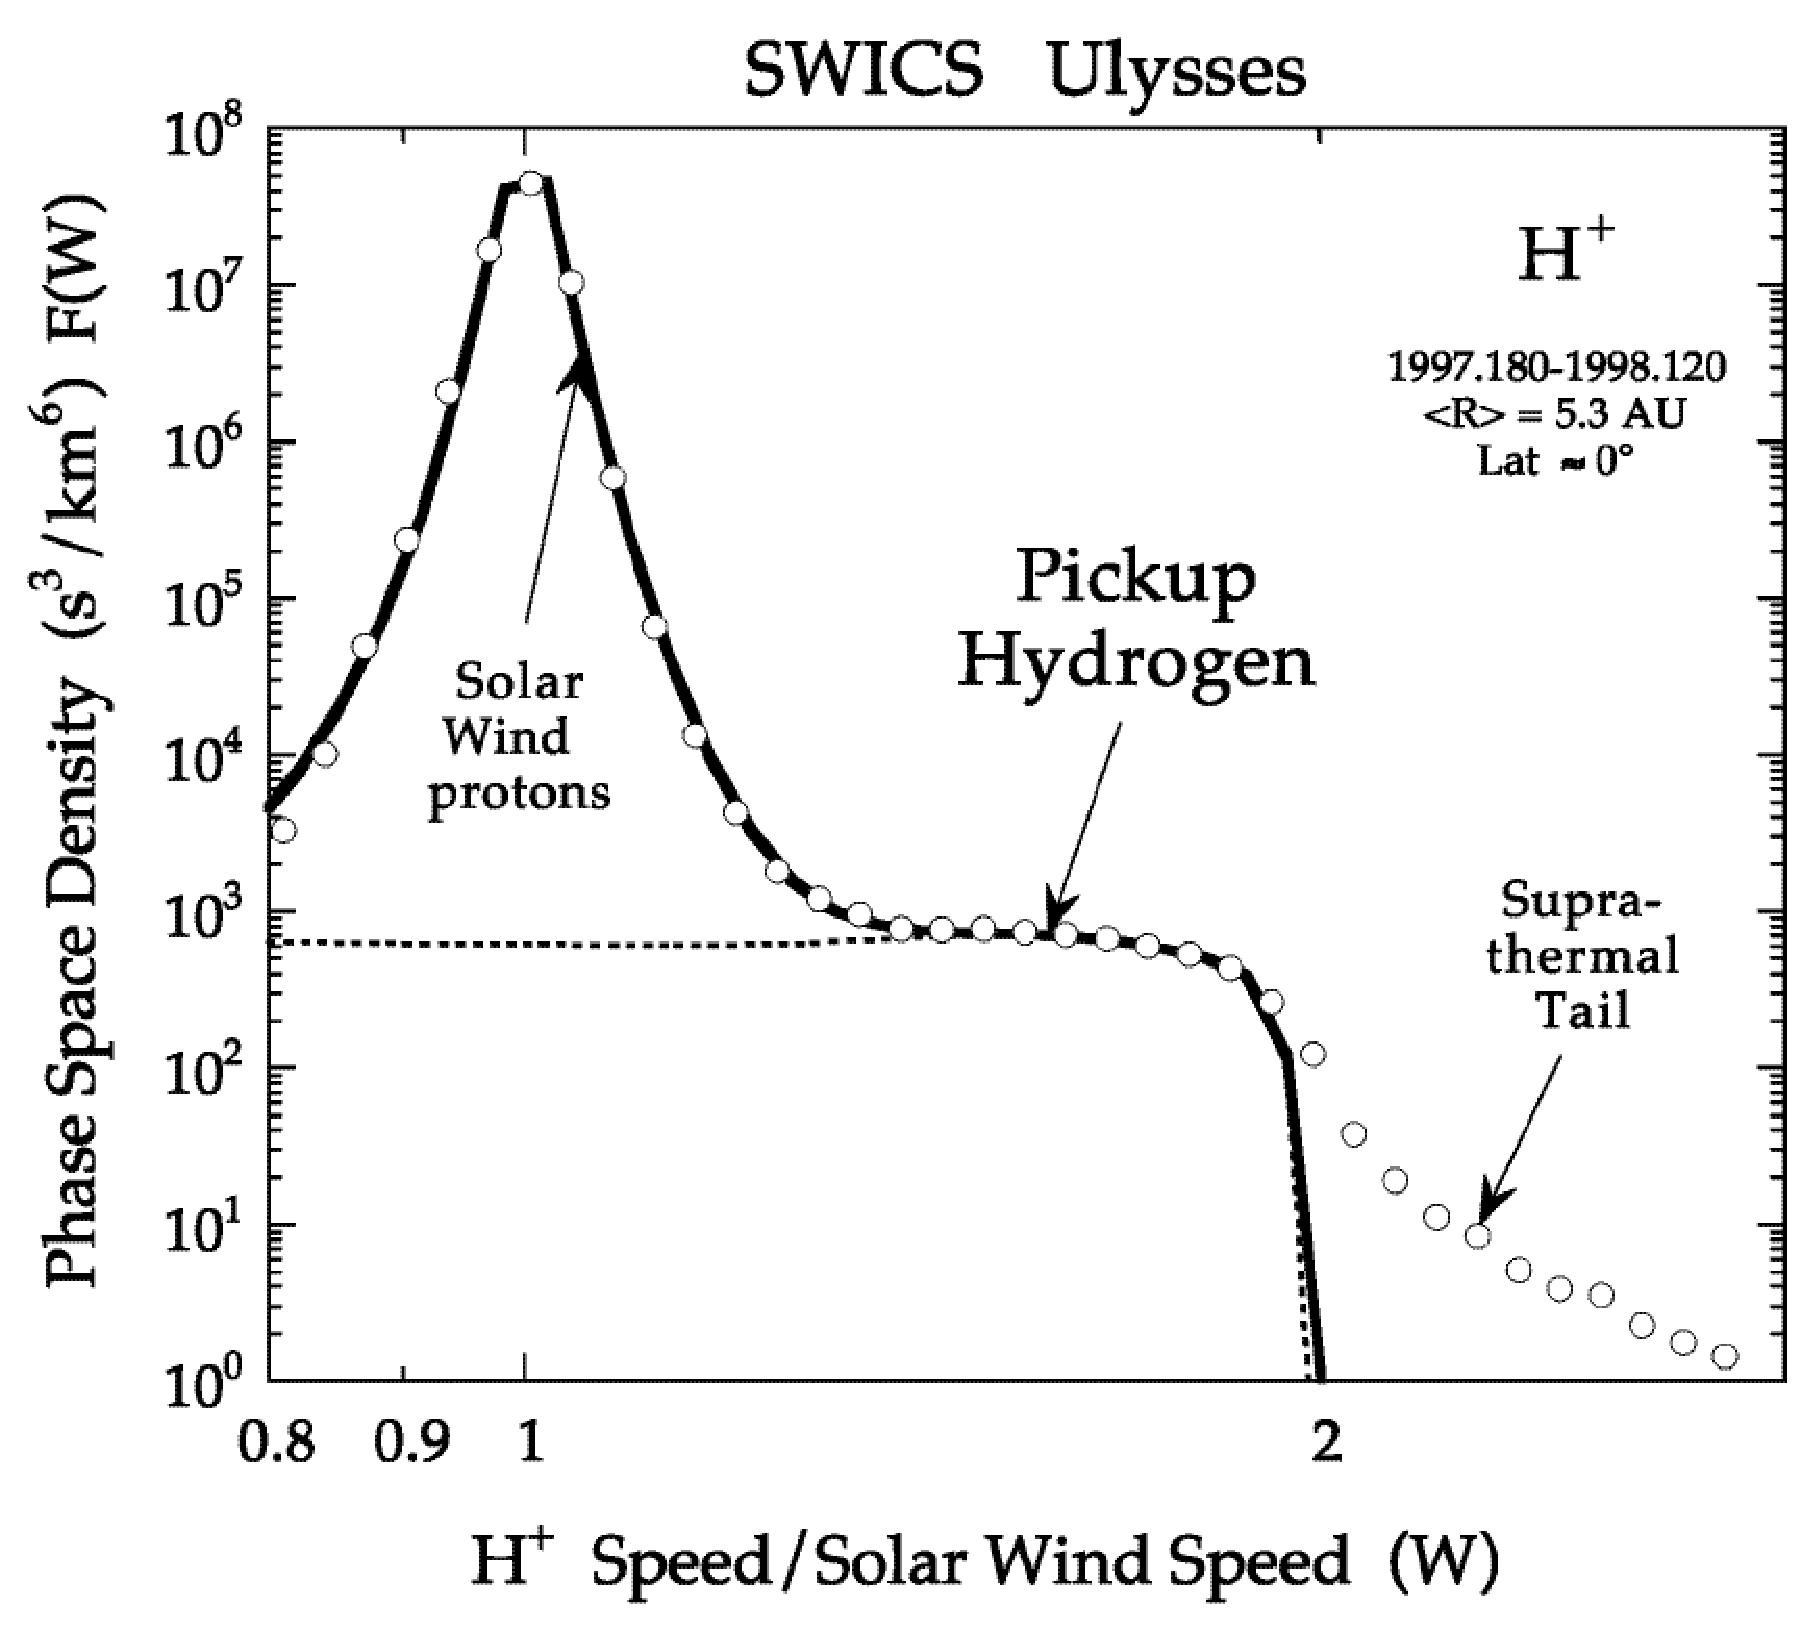
\includegraphics[width=.65\textwidth]{Chap2/H_Distribution}
  \caption[Example of proton distributions for the quiet solar wind near 5 AU.]{Example of proton distributions for the quiet solar wind near 5 AU. Shown are the bulk distribution of the solar wind, the interstellar pickup ions that drop off at twice the solar wind speed, and the high-energy protons that make up the suprathermal tail. Figure from \citet{gloeckler01b}.}
  \label{fig:H_Distribution}
\end{figure}

\section{The Solar Wind}
\label{Solar Wind}

\subsection{Current Knowledge}
\label{SW Current Knowledge}
While he was not the first to postulate its existence, the physics of the solar wind was first explained by Eugene Parker in 1958 \citep{parker58}. Beginning with subsonic speeds close to the Sun, plasma accelerates away from the solar surface and reaches supersonic speeds in the corona. It continues to expand in a radial direction outward until it interacts with the material in interstellar space at the edge of the heliosphere, the Sun's sphere of influence. The wind draws the solar magnetic field along with it, creating spiral-shaped field lines as the Sun rotates \citep{parker59}. Mankind's understanding of the processes that govern the solar wind has increased as spacecraft have taken in situ measurements, but there are still some properties that remain unexplained, such as the precise origin of certain types of wind, as discussed below.

The solar wind travels a distance of one \ac{AU} before reaching Earth's orbit, where most of the current measurements have been taken (Table~\ref{tab:solar wind}). It is generally divided into two components, commonly referred to as the ``fast'' and ``slow'' solar wind. Originally, these terms were used to differentiate the wind by the speed with which it traveled, but more recent studies have shown that the two types of wind are more efficiently distinguished by their charge state composition (e.g., O$^{7+}$/O$^{6+}$) since the plasma can change speeds as it flows through space \citep{geiss95b, gloeckler03a}. Rather than the terms ``fast'' and ``slow'', more appropriate labels are descriptive of the wind's origin: ``coronal hole'' and ``streamer'' wind. These two types of wind are generated by different processes and have different compositions, temperatures, speeds, and origins.
\begin{table}[htbp]
	\centering
		\begin{tabular}{l|c|c}
		                                                               & Coronal Hole Wind & Streamer Wind     \\ \hline
      bulk speed \footnotesize{$\left(\text{km s}^{-1}\right)$}    & 750               & 400               \\ \hline
      thermal speed \footnotesize{$\left(\text{km s}^{-1}\right)$} & 32                & 35                \\ \hline
      H$^+$ density \footnotesize{$\left(\text{cm}^{-3}\right)$}   & 2.5               & 8.7               \\ \hline
      frozen-in temperature \footnotesize{$\left(\text{K}\right)$} & 8 x 10$^5$        & 1.4--1.6 x 10$^6$ \\ \hline

		\end{tabular}
	\caption[Average characteristics of the solar wind at 1 AU.]{Average characteristics of the solar wind at 1 AU. The temperature is derived from the freeze-in temperature of C$^{6+}$/C$^{5+}$, which freezes in near the solar wind source altitude. Data compiled from \citet{vonsteiger95, gloeckler98a, ipavich98, mccomas00, feldman05}.}
	\label{tab:solar wind}
\end{table}

As solar wind ions escape from the photosphere and travel up through the corona, they experience collisions with energetic electrons that ionize them to different degrees. As they travel farther through the corona, continuously accelerating, the density of coronal electrons decreases and the particles experience fewer collisions. When the timescale for ionization or recombination becomes longer than the timescale of the solar wind to expand through a density scale height, the charge state of the ion is said to be ``frozen in,'' branding the ion with the coronal region and electron temperature of its origin \citep{hundhausen68}. The streamer wind has a distinct characteristic of being enriched in elements with a low ($\le$ 10 eV) \ac{FIP} by a factor of 3--4 over the photospheric value. The coronal hole wind does not show this density enhancement, and measurements have revealed abundances of low-\ac{FIP} elements that match ratios in the photosphere \citep{vonsteiger93}. The streamer wind also has a higher and more variable freeze-in temperature than the coronal hole wind. One explanation for this describes solar plasma trapped and heated in large coronal loops that are eventually opened by interchange reconnection, releasing the plasma \citep{gosling95, fisk98, fisk99a}.

The coronal hole wind originates in the open flux regions of the Sun, which contain low-density plasma and concentrations of magnetic flux that are all the same polarity. During solar minimum these regions are clustered around the poles of the Sun, while during solar maximum they appear at all latitudes. Plasma in open flux regions is also released from flux loops, but the high concentration of open flux increases the probability that the loops will open before they can heat and fractionate the plasma. The anti-correlation between freeze-in temperature and solar wind speed shown in Table~\ref{tab:solar wind} can be interpreted in a simplistic way as a sign of different sized loops. The long-lived loops that produce the streamer wind will expand and rise slowly into the corona, where the temperatures are hotter, before being opened \citep{fisk98, fisk01a}. The short-lived loops that yield the coronal hole wind are opened while they are still small and close to the cooler surface \citep{fisk99a, fisk03, wimmer03b}.

\startappendices
 \appendix{Two-Dimensional Crank-Nicolson Scheme for a Uniform Spherical Grid}
 \label{app:CN Scheme}
 For the diffusion process, The equation was solved using a two-dimensional implicit Crank-Nicolson scheme, which is unconditionally stable and second-order accurate in both time and space \citep{crank47}. In the conventional notation, the two-dimensional numerical scheme using central differencing can be written for a uniform Cartesian grid as 
\begin{eqnarray}
\nonumber\left(1+2\mu\right)u^{t+1}_{i,j}-\frac{\mu}{2}\left(u^{t+1}_{i+1,j}+u^{t+1}_{i-1,j}+u^{t+1}_{i,j+1}+u^{t+1}_{i,j-1}\right)\\
=\left(1-2\mu\right)u^{t}_{i,j}+\frac{\mu}{2}\left(u^{t}_{i+1,j}+u^{t}_{i-1,j}+u^{t}_{i,j+1}+u^{t}_{i,j-1}\right),
\end{eqnarray}

\noindent where $u^{t}_{i,j}$ is the value of the parameter undergoing the diffusion ($B_{r}$ in this case) at position $(i, j)$ at time \textit{t}. The von Neumann number on a uniform grid is $\mu=\xi{\Delta}t/\left({\Delta}x\right)^{2}$, where the size of the grid square is $\Delta x$ on each side, and the diffusion coefficient $\xi$ describes the speed at which the mathematical diffusion takes place. When deriving the two-dimensional Crank-Nicolson scheme in spherical coordinates, the von Neumann number is written as $\mu=\xi{\Delta}t/\left(r\Delta\theta\right)^{2}$, where $\Delta\theta=\Delta\phi$, and the cosine is replaced by the central difference of the sine to remain consistent with the discrete nature of the other terms. Care must be taken at the poles, where the central differencing is replaced by forward or backward differencing. To keep second-order accuracy with forward or backward differencing, the series must be carried out to higher-order terms in the derivation. The two-dimensional numerical scheme using central differencing can be written for a uniform spherical grid as
\begin{multline}
\left(1+\mu+\frac{\mu}{\sin^{2}\theta_{i,j}}\right)u^{t+1}_{i,j}-\frac{\mu}{2}\left[1+\frac{\left(\sin\theta_{i+1,j}-\sin\theta_{i-1,j}\right)}{4\sin\theta_{i,j}}\right]u^{t+1}_{i+1,j}\\
 -\frac{\mu}{2}\left[1-\frac{\left(\sin\theta_{i+1,j}-\sin\theta_{i-1,j}\right)}{4\sin\theta_{i,j}}\right]u^{t+1}_{i-1,j}-\frac{\mu}{2}\frac{1}{\sin^{2}\theta_{i,j}}u^{t+1}_{i,j+1}-\frac{\mu}{2}\frac{1}{\sin^{2}\theta_{i,j}}u^{t+1}_{i,j-1}\\
 =\left(1-\mu-\frac{\mu}{\sin^{2}\theta_{i,j}}\right)u^{t+1}_{i,j}+\frac{\mu}{2}\left[1+\frac{\left(\sin\theta_{i+1,j}-\sin\theta_{i-1,j}\right)}{4\sin\theta_{i,j}}\right]u^{t+1}_{i+1,j}\\
 +\frac{\mu}{2}\left[1-\frac{\left(\sin\theta_{i+1,j}-\sin\theta_{i-1,j}\right)}{4\sin\theta_{i,j}}\right]u^{t+1}_{i-1,j}+\frac{\mu}{2}\frac{1}{\sin^{2}\theta_{i,j}}u^{t+1}_{i,j+1}+\frac{\mu}{2}\frac{1}{\sin^{2}\theta_{i,j}}u^{t+1}_{i,j-1}.
 \label{CN Spherical}
\end{multline}

Although it is unconditionally stable, a marching scheme such as this will depend on the value of $\mu$ for its accuracy. A lower choice of $\mu$ will lead to a more accurate solution at the expense of computational resources (i.e., a smaller time step ${\Delta}t$), while a higher value of $\mu$ will arrive at a solution more rapidly but with less accuracy (a larger time step). In this model, the value of the coefficient $\xi$ describes the speed of the mathematical relaxation and, since it does not describe a physical process, can be chosen arbitrarily. Thus the only restriction for this scheme will lie in keeping $\mu$ small for accuracy and assigning either $\xi$ or ${\Delta}t$. It can be seen that when $\mu$ is held constant, any choice for either $\xi$ or ${\Delta}t$ will lead to the same solution. A value of $\mu=1/4$ was chosen, with an arbitrary time step of ${\Delta}t=0.1$ s, and studied several different grid resolutions, with a grid size of 2.5$^\circ$ x 2.5$^\circ$ (72 x 144 grid spaces) on a uniform spherical grid used for the comparisons in this paper. The relaxation was allowed to continue on a sphere of $r=R_{\sun}$ until the difference in magnetic field magnitude between any cell and its neighbor was of order $10^{-1}{\mu}T$.
 
\startbibliography
 \begin{singlespace} % Bibliography must be single spaced
  \bibliography{References}   % Use the BibTeX file ``References.bib''.
 \end{singlespace}

% An external Abstract that can be printed at the end of the document, 
% for separate submission to Rackham. Comment it out when not needed. - jg
%\startextabstractpage
%{The Title of Your Dissertation}{Your Name}{Chair: Albert Einstein}
%This template conforms to University of Michigan abstract and dissertation format guidelines as of September 2008. It is an update to a template that has been floating around among grad students here for about 20 years. The main components are the thesis.tex file and the rac.sty file, the latter of which should not need any modification. If BibTeX is used (and for a dissertation, it should be), then References.bib is also needed. If a list of acronyms is desired, make all additions in abbr.tex and read acronym.pdf on ctan.org for details on how to call them in the text. Other files in this template that may be helpful, but don't necessarily need to be used include a style file that formats your bibliography in AGU format (agu04.bst) and a style file that allows you to use abbreviations for journal names (aas\_macros.sty) when typing out the bibliography. This will be necessary if you grab BibTeX information from places like the NASA ADS, which sometimes uses journal name abbreviations. It is useful to separate chapters into their own subfolders, with each folder containing the chapter's .tex file as well as all associated figures. For the figures, just call the name of the file, without the suffix (i.e., includegraphics\{Chap5/LabSetup\}) and the graphicx package will figure out what type of file it is. To compile to pdf, some format other than .eps must be used with the figures. To compile to ps, the figures need to be in ps or eps. If using \LaTeX\, in a Windows environment, there are several different editors and programs that can be used. One set that is known to work well is the following, which can each be found with a simple web search and which should be installed in this order: a Perl distribution such as ActivePerl, a \TeX\, distribution such as MikTex, a \LaTeX\, editor such as TeXnicCenter, a postscript interpreter like Ghostscript, and a postscript viewer like GSView. I included a few pages of sample code in chapter 2 to help you get started, including code for writing equations, citations, abbreviations, tables, and calling graphics. Always be sure to compile your thesis.tex file a couple of times to get the references and page numbering updated. Good luck. -jg
%\label{ExtAbstract}

\end{document}
